\documentclass[11pt]{amsart}

\usepackage[margin=1.15in]{geometry}
\usepackage{amsmath,amssymb,amsthm,mathtools}
\usepackage{booktabs,array}
\usepackage{graphicx}
\usepackage{microtype}
\usepackage[hidelinks]{hyperref}
\usepackage[capitalise,nameinlink]{cleveref}

\newtheorem{theorem}{Theorem}[section]
\newtheorem{proposition}[theorem]{Proposition}
\newtheorem{lemma}[theorem]{Lemma}
\newtheorem{corollary}[theorem]{Corollary}
\newtheorem{conjecture}[theorem]{Conjecture}
\theoremstyle{definition}
\newtheorem{definition}[theorem]{Definition}
\theoremstyle{remark}
\newtheorem{remark}[theorem]{Remark}

\newcommand{\PP}{\mathcal{P}}
\newcommand{\Ls}{\mathcal{L}}
\newcommand{\Us}{\mathcal{U}}
\newcommand{\Es}{\mathcal{E}}
\newcommand{\Sg}{\mathfrak{S}}
\newcommand{\Z}{\mathbb{Z}}
\newcommand{\N}{\mathbb{N}}

\title[Goldbach problems for Polignac families]{Goldbach problems for Polignac families:\\ twin, cousin and sexy summands}

\author{Paul Bilokon}
\address{Department of Mathematics, Imperial College London, London, United Kingdom; and Thalesians Ltd, London, United Kingdom}
\email{paul@thalesians.com}

\date{19 October 2026}

\subjclass[2020]{Primary 11P32; Secondary 11N05, 11Y11}
\keywords{Goldbach problem, twin primes, cousin primes, sexy primes, Polignac conjecture, Hardy--Littlewood conjecture, singular series}

\begin{document}

\begin{abstract}
For an even integer $d$, let $\PP_d$ be the set of primes $p$ such that $p-d$ or $p+d$ is also prime; thus $\PP_2$, $\PP_4$ and $\PP_6$ are the twin, cousin and sexy primes. We study the binary problem of representing an even integer $n$ as $p+q$ with $p\in\PP_a$ and $q\in\PP_b$, which for $a=b=2$ is the twin-prime Goldbach problem of Zwillinger and Dubner. By an exact, integer-only witness search we determine the exceptional sets for all six pairings of twin, cousin and sexy primes up to $10^8$, and for all $120$ pairs of gaps $a,b\le 30$ up to $10^7$. Every even $n\ge 6$ is the sum of a twin prime and a cousin prime in this range, whereas twin$+$twin and cousin$+$cousin have $34$ and $36$ exceptions, the largest being $4208$ and $2952$. We prove a structure theorem modulo~$3$ that explains this contrast: when $3\nmid a$, the representations of $s$, $s+a$, $s+2a$ are locked together in the exact ratio $1:2:1$, so equal-gap exceptions occur in arithmetic triples, while for $a\ne b$ the class $n\equiv 0\pmod 3$ has two independent routes. As a corollary, the twin-prime Goldbach problem for multiples of $6$ is equivalent to a Goldbach problem for the index set $\{k:6k\pm1\text{ both prime}\}$. We formulate a Hardy--Littlewood type conjecture for $r_{a,b}(n)$, prove that its singular series is bounded below by an explicit absolute constant $c_0\approx 4.1512$ (halved when $a=b$), and show that the prediction, refined by inclusion--exclusion, matches the data to within $1\%$ near $10^7$ and reproduces the number of observed exceptions. Any proof of the existence part for a single pair $(a,b)$ would establish Polignac's conjecture for gap $a$ or gap $b$.
\end{abstract}

\maketitle

\section{Introduction}

Goldbach's conjecture asserts that every even integer $n\ge 4$ is a sum of two primes. It has been verified up to $4\cdot 10^{18}$ \cite{OliveiraESilva2014}, it holds for almost all even $n$ \cite{MontgomeryVaughan1975}, and Chen proved that every sufficiently large even $n$ is the sum of a prime and a number with at most two prime factors \cite{Chen1973}; a complete proof remains out of reach. A natural strengthening restricts the summands to primes with additional arithmetic structure. In 1979 Zwillinger \cite{Zwillinger1979} checked every even number up to $10^6$ for a representation as a sum of two primes each belonging to a twin-prime pair, and found $33$ exceptions, all below $5000$. Dubner \cite{Dubner2000} conjectured that $4208$ is the largest such exception; the list is sequence A007534 of the OEIS, which records that there are no further exceptions below $10^{11}$ \cite{OEIS_A007534}. A recent preprint considers the intermediate problem of a prime plus a twin prime \cite{Pandey2026}.

Twin primes are the first of the families singled out by Polignac's conjecture \cite{Polignac1849}, which predicts infinitely many prime pairs with any prescribed even difference. This suggests the following general question.

\begin{definition}\label{def:Pd}
For even $d\ge 2$ let
\[
\PP_d=\{p \text{ prime}: p-d \text{ or } p+d \text{ is prime}\}.
\]
For even $a,b\ge 2$ and even $n$, let $r_{a,b}(n)$ be the number of ordered pairs $(p,q)\in\PP_a\times\PP_b$ with $p+q=n$, and let
\[
E_{a,b}=\{n\ge 4 \text{ even}: r_{a,b}(n)=0\},\qquad n_0(a,b)=2+\max E_{a,b},
\]
so that $n_0(a,b)$ is the least $n_0$ such that every even $n\ge n_0$ is represented (if $E_{a,b}$ is finite).
\end{definition}

We call $\PP_2$, $\PP_4$ and $\PP_6$ the \emph{twin}, \emph{cousin} and \emph{sexy} primes. Note that $3\in\PP_2\cap\PP_4$ (via $5$ and $7$) but $3\notin\PP_6$, and $2$ lies in no $\PP_d$. The twin-prime Goldbach problem is the case $a=b=2$.

\subsection*{Results}
Our contributions are as follows.

\begin{enumerate}
\item \emph{Exact computations} (\cref{sec:computations}). We determine $E_{a,b}\cap[4,10^8]$ for the six pairings of twin, cousin and sexy primes and $E_{a,b}\cap[4,10^7]$ for all pairs $2\le a\le b\le 30$, using an integer-only witness search. The thresholds are summarised in \cref{tab:six,tab:grid}. In particular, every even $n\ge 6$ up to $10^8$ is the sum of a twin prime and a cousin prime, while the twin$+$twin and cousin$+$cousin problems have $34$ and $36$ exceptions.

\item \emph{A structure theorem modulo $3$} (\cref{sec:structure}). For $3\nmid ab$ we express $r_{a,b}$, up to a bounded error, through a single convolution $N_{a,b}$ of ``lower pair members'' (\cref{thm:decomposition}). For $a=b$ this gives the exact identity $r^*(s):r^*(s+a):r^*(s+2a)=1:2:1$, which forces equal-gap exceptions to occur in arithmetic triples (\cref{cor:triples}), and it shows that the twin-prime Goldbach problem for multiples of $6$ is equivalent to a Goldbach problem for the set of indices $k$ with $6k\pm1$ prime (\cref{cor:index}). For $a\neq b$ the residue class $0\bmod 3$ has two independent routes (\cref{cor:mixed}), which the data confirm.

\item \emph{A conjecture with explicit singular series} (\cref{sec:heuristic}). We state a Hardy--Littlewood type asymptotic for $r_{a,b}(n)$ (\cref{conj:main}) and prove that its singular series is bounded below by an absolute constant $c_0\approx 4.1512$, halved when $a=b$ (\cref{lem:positivity}). There is therefore no local obstruction for any pair of gaps.

\item \emph{Numerical evidence} (\cref{sec:evidence}). The prediction, refined by inclusion--exclusion over the membership conditions, matches $r_{a,b}(n)$ to within $1\%$ for $n$ near $10^7$ for all six pairings, with correlation above $0.998$. A Poisson model built from it predicts $16.3$ and $16.2$ exceptions above $1000$ for twin$+$twin and cousin$+$cousin; the observed numbers are $18$ and $19$.

\item \emph{Limits} (\cref{sec:discussion}). The existence statement for any single pair $(a,b)$ implies Polignac's conjecture for gap $a$ or gap $b$ (\cref{prop:polignac}), so it is at least as hard as the twin-prime conjecture in the case $a=b=2$.
\end{enumerate}

\section{Computations}\label{sec:computations}

\subsection{Method}
We sieve the primes up to $N+\max(a,b)$ and form the indicator arrays of $\PP_a$ and $\PP_b$ on $[0,N]$. Let $U$ be the set of even $n\in[4,N]$, and process the elements $p\in\PP_a$ in increasing order. At each step we remove from $U$ every $n$ with $n-p\in\PP_b$, recording $p$ as the minimal witness for $n$; and we declare exceptional every $n\in U$ with $n<p+\min\PP_b$, since no later element of $\PP_a$ can represent it. The procedure stops when $U$ is empty. It uses integer arithmetic only, every non-exception receives an explicit witness, and every exception is certified by exhaustion. For the statistics of $r_{a,b}(n)$ in \cref{sec:evidence} we compute the full convolution with a fast Fourier transform in double precision and round to integers; on the overlapping range the two methods give identical exceptional sets. The exceptional set for $(2,2)$ coincides with A007534 \cite{OEIS_A007534}, which serves as a check.

\subsection{Twin, cousin and sexy pairings}

\begin{theorem}\label{thm:six}
For the six pairings of $\PP_2,\PP_4,\PP_6$, the sets $E_{a,b}\cap[4,10^8]$ are as follows:
\begin{align*}
E_{2,4}&=\{4\}, & E_{2,6}&=E_{4,6}=\{4,6\}, & E_{6,6}&=\{4,6,8\},
\end{align*}
\begin{multline*}
E_{2,2}=\{4,94,96,98,400,402,404,514,516,518,784,786,788,904,906,908,\\1114,1116,1118,1144,1146,1148,1264,1266,1268,1354,1356,1358,\\3244,3246,3248,4204,4206,4208\},
\end{multline*}
\begin{multline*}
E_{4,4}=\{4,8,12,68,72,76,278,282,286,638,642,644,648,652,908,912,916,\\1058,1062,1066,1328,1332,1336,1418,1422,2114,2118,2122,\\2294,2298,2302,2528,2532,2536,2948,2952\}.
\end{multline*}
\end{theorem}

\begin{proof}
Exhaustive computation by the method above.
\end{proof}

\begin{table}[t]
\centering
\caption{The six pairings of twin ($a=2$), cousin ($a=4$) and sexy ($a=6$) primes, verified exactly to $10^8$. The last column gives the largest minimal witness: the largest value, over even $n\in[n_0,10^8]$, of the least $p\in\PP_a$ with $n-p\in\PP_b$.}
\label{tab:six}
\begin{tabular}{lrrr}
\toprule
Pairing $(a,b)$ & $n_0(a,b)$ & $|E_{a,b}|$ & largest minimal witness $p$ (at $n$) \\
\midrule
twin $+$ twin $(2,2)$ & 4210 & 34 & 117\,703 \ (64\,752\,656) \\
cousin $+$ cousin $(4,4)$ & 2954 & 36 & 120\,623 \ (80\,759\,296) \\
sexy $+$ sexy $(6,6)$ & 10 & 3 & 26\,833 \ (50\,059\,412) \\
twin $+$ cousin $(2,4)$ & 6 & 1 & 115\,021 \ (94\,270\,994) \\
twin $+$ sexy $(2,6)$ & 8 & 2 & 33\,329 \ (89\,769\,676) \\
cousin $+$ sexy $(4,6)$ & 8 & 2 & 40\,849 \ (59\,836\,418) \\
\bottomrule
\end{tabular}
\end{table}

The equal-gap exceptional sets have a visible structure: apart from a few small cases, they consist of triples $\{s,s+a,s+2a\}$, such as $\{94,96,98\}$ for $a=2$ and $\{68,72,76\}$ for $a=4$. The occasional incomplete triple, such as $\{1418,1422\}$ in $E_{4,4}$, arises because $1426=3+1423$ with $1423\in\PP_4$. \Cref{sec:structure} explains this.

\subsection{All gaps up to 30}
\Cref{tab:grid} gives $n_0(a,b)$ for all $2\le a\le b\le 30$, computed exactly to $10^7$. Two patterns stand out.

\begin{itemize}
\item If $3\mid a$ or $3\mid b$, then $n_0(a,b)\le 58$ (the maximum, $58$, occurs for $(12,12)$).
\item If $3\nmid ab$, the large thresholds occur on the diagonal $a=b$: $n_0(a,a)$ ranges from $666$ $(a=28)$ to $5736$ $(a=16)$, except for $a\in\{10,20\}$ where $n_0=30$ and $40$; there the factor $(\ell-1)/(\ell-2)=4/3$ at $\ell=5$ raises the density of $\PP_a$. Off the diagonal large thresholds are rarer: the largest are $1944$ $(2,16)$, $1356$ $(2,28)$ and $1300$ $(4,26)$, while for instance $n_0(2,4)=6$.
\end{itemize}

\begin{table}[t]
\centering
\caption{Thresholds $n_0(a,b)$ for $2\le a\le b\le 30$, verified exactly to $10^7$. Bold entries exceed $500$.}
\label{tab:grid}
\small
\setlength{\tabcolsep}{3.2pt}
\begin{tabular}{r*{15}{c}}
\toprule
$a\backslash b$ & 2 & 4 & 6 & 8 & 10 & 12 & 14 & 16 & 18 & 20 & 22 & 24 & 26 & 28 & 30 \\ \midrule
2 & \textbf{4210} & 6 & 8 & 6 & 6 & 8 & 6 & \textbf{1944} & 8 & 14 & 30 & 8 & 28 & \textbf{1356} & 10 \\
4 &  & \textbf{2954} & 8 & 6 & 14 & 8 & 6 & \textbf{654} & 12 & 34 & 390 & 8 & \textbf{1300} & 30 & 14 \\
6 &  &  & 10 & 8 & 8 & 10 & 8 & 8 & 16 & 14 & 30 & 10 & 8 & 30 & 12 \\
8 &  &  &  & \textbf{2326} & 6 & 8 & 14 & 328 & 22 & 40 & 168 & 16 & 40 & 30 & 10 \\
10 &  &  &  &  & 30 & 18 & 16 & 30 & 12 & 14 & 30 & 8 & 6 & 54 & 24 \\
12 &  &  &  &  &  & 58 & 20 & 18 & 16 & 14 & 34 & 10 & 8 & 42 & 12 \\
14 &  &  &  &  &  &  & \textbf{1100} & 140 & 22 & 40 & 30 & 16 & 40 & 30 & 10 \\
16 &  &  &  &  &  &  &  & \textbf{5736} & 12 & 30 & 48 & 8 & 6 & 60 & 30 \\
18 &  &  &  &  &  &  &  &  & 22 & 40 & 30 & 16 & 40 & 30 & 16 \\
20 &  &  &  &  &  &  &  &  &  & 40 & 30 & 16 & 40 & 40 & 14 \\
22 &  &  &  &  &  &  &  &  &  &  & \textbf{2160} & 42 & 30 & 60 & 36 \\
24 &  &  &  &  &  &  &  &  &  &  &  & 18 & 16 & 30 & 12 \\
26 &  &  &  &  &  &  &  &  &  &  &  &  & \textbf{4390} & 166 & 10 \\
28 &  &  &  &  &  &  &  &  &  &  &  &  &  & \textbf{666} & 30 \\
30 &  &  &  &  &  &  &  &  &  &  &  &  &  &  & 34 \\
\bottomrule
\end{tabular}
\end{table}

\section{Structure modulo 3}\label{sec:structure}

We begin with the elementary observation that limits what can be proved.

\begin{proposition}\label{prop:polignac}
If $E_{a,b}$ is finite, then $\PP_a$ or $\PP_b$ is infinite; that is, there are infinitely many prime pairs with difference $a$ or infinitely many with difference $b$. In particular, finiteness of $E_{2,2}$ implies the twin-prime conjecture.
\end{proposition}

\begin{proof}
If $\PP_a$ and $\PP_b$ are both finite then so is $\PP_a+\PP_b$, which then cannot contain all sufficiently large even integers. Finally, $\PP_d$ is infinite if and only if there are infinitely many primes $p$ with $p+d$ prime, since every element of $\PP_d$ is a member of such a pair.
\end{proof}

From now on fix even $a,b\ge 2$. Primes $p>3$ lie in the classes $\pm1\bmod 3$, and when $3\nmid a$ the two members of a pair $(p,p+a)$ with $p>3$ are forced into opposite classes. This rigidity is the source of the structure below.

\begin{definition}
For even $a$ with $3\nmid a$ let
\[
\Ls_a=\{p>3: p \text{ and } p+a \text{ prime}\},\qquad \Us_a=\Ls_a+a,\qquad \Es_a=\PP_a\setminus(\Ls_a\cup\Us_a).
\]
\end{definition}

\begin{lemma}\label{lem:classes}
Let $3\nmid a$. Then $\Ls_a\subseteq\{x\equiv a\pmod 3\}$ and $\Us_a\subseteq\{x\equiv -a\pmod 3\}$; in particular $\Ls_a\cap\Us_a=\varnothing$. Moreover $\Es_a\subseteq\{3,a+3\}$.
\end{lemma}

\begin{proof}
If $p\in\Ls_a$ then $p\not\equiv 0$ and $p+a\not\equiv 0\pmod 3$, so $p\not\equiv -a$; since $a\not\equiv 0$, the only remaining nonzero class is $p\equiv a$. Hence $p+a\equiv 2a\equiv -a$, which proves the first two inclusions.

Now let $p\in\PP_a\setminus(\Ls_a\cup\Us_a)$. Since $2+a$ is even and greater than $2$, and $2-a\le 0$, we have $2\notin\PP_a$, so $p$ is odd. Suppose $p>3$. If $p+a$ were prime then $p\in\Ls_a$, so $p-a$ is prime. If $p-a>3$ then $p-a\in\Ls_a$ and $p\in\Us_a$, a contradiction; and $p-a$ is odd and prime, so $p-a=3$. Hence $p\in\{3,a+3\}$.
\end{proof}

Write $\Ls=\Ls_a$, $\Us=\Us_a$ and similarly $\Ls'=\Ls_b$, $\Us'=\Us_b$, and define for integers $m$
\begin{align*}
N_{a,b}(m)&=\#\{(x,y)\in\Ls_a\times\Ls_b: x+y=m\},\\
r^*_{a,b}(n)&=\#\{(p,q)\in(\Ls\cup\Us)\times(\Ls'\cup\Us'): p+q=n\}.
\end{align*}

\begin{theorem}\label{thm:decomposition}
Let $a,b$ be even with $3\nmid ab$. Then for every even $n$:
\begin{enumerate}
\item $0\le r_{a,b}(n)-r^*_{a,b}(n)\le |\Es_a|+|\Es_b|\le 4$;
\item $r^*_{a,b}(n)=N_{a,b}(n)+N_{a,b}(n-a)+N_{a,b}(n-b)+N_{a,b}(n-a-b)$;
\item $N_{a,b}(m)=0$ unless $m\equiv a+b\pmod 3$. Consequently:
\begin{itemize}
\item if $a\equiv b\pmod 3$: $r^*(n)=N(n)$ for $n\equiv -a$; $r^*(n)=N(n-a)+N(n-b)$ for $n\equiv 0$; $r^*(n)=N(n-a-b)$ for $n\equiv a\pmod 3$;
\item if $a\equiv -b\pmod 3$: $r^*(n)=N(n)+N(n-a-b)$ for $n\equiv 0$; $r^*(n)=N(n-a)$ for $n\equiv a$; $r^*(n)=N(n-b)$ for $n\equiv -a\pmod 3$.
\end{itemize}
\end{enumerate}
\end{theorem}

\begin{proof}
(1) By \cref{lem:classes}, $\PP_a$ is the disjoint union of $\Ls\cup\Us$ and $\Es_a$, and similarly for $b$. A representation counted by $r_{a,b}(n)$ but not by $r^*_{a,b}(n)$ has $p\in\Es_a$ or $q\in\Es_b$; for each such fixed $p$ (respectively $q$) there is at most one partner.

(2) The four products $\Ls\times\Ls'$, $\Ls\times\Us'$, $\Us\times\Ls'$, $\Us\times\Us'$ partition the pairs counted by $r^*$, since $\Ls\cap\Us=\Ls'\cap\Us'=\varnothing$. Translating the second coordinate by $-b$, the first by $-a$, or both, maps them bijectively onto the pairs in $\Ls\times\Ls'$ with sums $n$, $n-b$, $n-a$, $n-a-b$ respectively.

(3) By \cref{lem:classes}, $x+y\equiv a+b\pmod 3$ for $(x,y)\in\Ls\times\Ls'$. If $a\equiv b$ then $a+b\equiv 2a\equiv -a$, and $n-c\equiv -a$ for $c\in\{0,a,b,a+b\}$ selects $c=0$ when $n\equiv -a$, $c\in\{a,b\}$ when $n\equiv 0$, and $c=a+b$ when $n\equiv -a+2a=a$. If $a\equiv -b$ then $a+b\equiv 0$, and the same bookkeeping gives the second case.
\end{proof}

\begin{corollary}[Equal gaps: locked triples]\label{cor:triples}
Let $3\nmid a$ and write $N=N_{a,a}$, $r^*=r^*_{a,a}$. For every $s\equiv -a\pmod 3$,
\[
r^*(s)=N(s),\qquad r^*(s+a)=2N(s),\qquad r^*(s+2a)=N(s).
\]
Hence the three numbers $s,s+a,s+2a$ are either all represented using $\Ls_a\cup\Us_a$ or none is, and
\[
E_{a,a}\subseteq\bigcup_{s\equiv -a\ (3),\ N(s)=0}\{s,\,s+a,\,s+2a\};
\]
an element of such a triple escapes $E_{a,a}$ only through a representation in which one summand lies in $\Es_a\subseteq\{3,a+3\}$.
\end{corollary}

\begin{proof}
Apply \cref{thm:decomposition}(2)--(3) with $b=a$: the two routes $N(n-a)$ and $N(n-b)$ for the class $n\equiv 0$ coincide. Then use part (1).
\end{proof}

For $a=b$ the residue class $0\bmod 3$ therefore receives a doubled count but no second chance: its representability is the same event as that of its two neighbours. For $a\ne b$ this degeneracy disappears.

\begin{corollary}[Distinct gaps: two routes]\label{cor:mixed}
Let $a\neq b$ with $3\nmid ab$. Then an even $n\equiv 0\pmod 3$ has $r^*_{a,b}(n)=0$ only if two values of $N_{a,b}$ at different arguments vanish simultaneously: $N(n-a)=N(n-b)=0$ if $a\equiv b\pmod 3$, and $N(n)=N(n-a-b)=0$ if $a\equiv -b\pmod 3$.
\end{corollary}

Heuristically, a vanishing value of $N$ is a rare event and two vanishing values at different arguments are rarer still, so exceptions for $a\neq b$ should avoid the class $0\bmod 3$. The data agree: among all pairs $a<b$ in $\{2,4,8,10,14,16,20,22,26,28\}$, the exceptions $n>a+b+6$ up to $10^7$ number $25$, and only one of them is divisible by $3$.

For the twin and cousin primes, \cref{cor:triples} becomes a Goldbach problem for an explicit set of integers.

\begin{corollary}[Index reformulation]\label{cor:index}
Let $K_2=\{k\ge1: 6k-1,\,6k+1 \text{ both prime}\}$ and $K_4=\{k\ge1: 6k+1,\,6k+5 \text{ both prime}\}$. For every $m\ge 2$,
\[
6m\in\PP_2+\PP_2 \iff m\in K_2+K_2,
\qquad
6m\in\PP_4+\PP_4 \iff m-1\in K_4+K_4 .
\]
In particular, every sufficiently large even integer is a sum of two twin primes if and only if every sufficiently large integer is a sum of two elements of $K_2$.
\end{corollary}

\begin{proof}
For $a=2$: an element $p\in\Ls_2$ satisfies $p\equiv 2\pmod 3$ and is odd, so $p=6k-1$ with $k\in K_2$, and conversely; thus $N_{2,2}(6m-2)=\#\{(k,j)\in K_2^2:k+j=m\}$. By \cref{cor:triples} with $s=6m-2\equiv -2\pmod 3$, $r^*_{2,2}(6m)=2N_{2,2}(6m-2)$. The only element of $\Es_2$ is $3$ (as $5\in\Ls_2$), and $6m=3+q$ would need $q=6m-3$, which for $m\ge2$ is divisible by $3$ and greater than $3$, hence not prime. So $r_{2,2}(6m)=r^*_{2,2}(6m)$, which proves the first equivalence.

For $a=4$: $p\in\Ls_4$ means $p\equiv 1\pmod 3$, so $p=6k+1$ with $k\in K_4$; thus $N_{4,4}(6M+2)=\#\{(k,j)\in K_4^2:k+j=M\}$. Taking $s=6(m-1)+2\equiv -4\pmod 3$ gives $r^*_{4,4}(6m)=r^*_{4,4}(s+4)=2N_{4,4}(6(m-1)+2)$. Here $\Es_4=\{3\}$ (since $7\in\Ls_4$), and $6m-3$ is again not prime for $m\ge 2$.

For the last statement: if $K_2+K_2$ contains every $m\ge m_0$, then by \cref{cor:triples} each triple $\{6m-2,6m,6m+2\}$ with $m\ge m_0$ is represented, and these triples cover all even $n\ge 6m_0-2$. Conversely, if every even $n\ge n_1$ is represented, apply the first equivalence to $n=6m$.
\end{proof}

Thus the exceptional triples of the twin-prime Goldbach problem correspond to the integers $m\notin K_2+K_2$; the last of them is $m=701$, giving $\{4204,4206,4208\}$. Similarly the triple $\{68,72,76\}$ of $E_{4,4}$ corresponds to $11\notin K_4+K_4$.

\begin{remark}
When $3\mid a$, the members of a pair $(p,p+a)$ lie in the same class modulo $3$, and both classes $\pm1$ occur. No analogue of \cref{lem:classes} holds, and the singular series in the next section is roughly doubled at the prime $3$. This is consistent with the small thresholds in the rows and columns of \cref{tab:grid} indexed by multiples of $3$.
\end{remark}

\section{A Hardy--Littlewood conjecture}\label{sec:heuristic}

\subsection{Heuristic}
Write $\mathbf 1_{\PP_a}(p)=\mathbf 1_{\mathrm{prime}}(p)\bigl(\mathbf 1_{\mathrm{prime}}(p+a)+\mathbf 1_{\mathrm{prime}}(p-a)-\mathbf 1_{\mathrm{prime}}(p+a)\mathbf 1_{\mathrm{prime}}(p-a)\bigr)$. Expanding $r_{a,b}(n)=\sum_{p}\mathbf 1_{\PP_a}(p)\mathbf 1_{\PP_b}(n-p)$ gives nine terms, each of which counts integers $x<n$ at which a fixed set of linear forms
\[
x+h\ (h\in H_1),\qquad n-x+k\ (k\in H_2),\qquad 0\in H_1\cap H_2,
\]
are simultaneously prime. The Hardy--Littlewood and Bateman--Horn heuristics \cite{HardyLittlewood1923,BatemanHorn1962} predict that such a count is asymptotic to
\begin{equation}\label{eq:BH}
C(H_1,H_2;n)\sum_{2\le x\le n-2}\frac{1}{(\log x)^{|H_1|}(\log(n-x))^{|H_2|}},\qquad
C=\prod_{\ell}\frac{1-\omega_\ell/\ell}{(1-1/\ell)^{|H_1|+|H_2|}},
\end{equation}
where $\omega_\ell$ is the number of residues of $\{-h:h\in H_1\}\cup\{n+k:k\in H_2\}$ modulo $\ell$. The four terms with $|H_1|=|H_2|=2$ dominate; the others carry an extra factor $1/\log n$. When $3\nmid a$, the term with $H_1=\{0,a,-a\}$ vanishes identically because $x-a,x,x+a$ cover all classes modulo $3$; when $3\mid a$ it is a genuine secondary term, corresponding to prime triples $(p-a,p,p+a)$.

\begin{definition}
For even $a,b$ and even $n>a+b$, define
\[
\Sg_{a,b}(n)=\theta_{a,b}\sum_{\varepsilon,\delta\in\{\pm1\}}\ \prod_{\ell}\beta_\ell(n;\varepsilon a,\delta b),\qquad
\beta_\ell=\frac{1-\omega_\ell/\ell}{(1-1/\ell)^4},
\]
where $\omega_\ell=\#\bigl(\{0,\,-\varepsilon a,\,n,\,n+\delta b\}\bmod\ell\bigr)$, $\theta_{a,b}=\tfrac12$ if $a=b$ and $\theta_{a,b}=1$ otherwise, and
\[
I(n)=\sum_{2\le x\le n-2}\frac{1}{(\log x)^2(\log(n-x))^2}\sim\frac{n}{(\log n)^4}.
\]
\end{definition}

The factor $\tfrac12$ for $a=b$ converts ordered pairs to unordered ones; we use unordered counts for $a=b$ in \cref{sec:evidence} and \cref{fig:counts}.

\begin{lemma}\label{lem:positivity}
Let $a,b$ be even and $n>a+b$ even. Each product $\prod_\ell\beta_\ell(n;\varepsilon a,\delta b)$ converges, and
\[
\Sg_{a,b}(n)\ \ge\ \theta_{a,b}\,c_0,\qquad
c_0=\frac{27}{2}\prod_{\ell\ge 5}\frac{1-4/\ell}{(1-1/\ell)^4}=4.15118\ldots
\]
In particular $\Sg_{a,b}(n)>0$: there is no local obstruction for any pair of gaps.
\end{lemma}

\begin{proof}
Fix $\varepsilon,\delta$. The residues $0,-\varepsilon a,n,n+\delta b$ have pairwise differences $\pm\varepsilon a$, $\pm\delta b$, $\pm n$, $\pm(n+\varepsilon a)$, $\pm(n+\delta b)$, $\pm(n+\varepsilon a+\delta b)$, all nonzero because $n>a+b$. Let $D$ be the product of these six differences. For $\ell\ge5$ with $\ell\nmid D$ we have $\omega_\ell=4$ and $\beta_\ell=1-6/\ell^2+O(\ell^{-3})$, so the product converges absolutely; for the finitely many $\ell\ge5$ dividing $D$ we have $\omega_\ell\le 4<\ell$, so $\beta_\ell>0$. In all cases $\beta_\ell\ge(1-4/\ell)(1-1/\ell)^{-4}$ for $\ell\ge5$.

At $\ell=2$ all four residues are even, so $\omega_2=1$ and $\beta_2=8$. At $\ell=3$ we have $\beta_3=0$ if $\omega_3=3$, and $\beta_3\ge(1-2/3)(2/3)^{-4}=27/16$ if $\omega_3\le2$. Hence every term with $\omega_3\le 2$ is at least $8\cdot\frac{27}{16}\prod_{\ell\ge5}(1-4/\ell)(1-1/\ell)^{-4}=c_0$, and all terms are nonnegative. It remains to find signs with $\omega_3\le2$, that is, with the set $\{0,-\varepsilon a,n,n+\delta b\}$ missing a class modulo $3$.

If $3\mid n$, the set is $\{0,-\varepsilon a,\delta b\}$ modulo $3$. If $3\mid a$ or $3\mid b$ it has at most two elements; otherwise choose the signs with $-\varepsilon a\equiv\delta b$. If $3\nmid n$, choose $\varepsilon$ with $-\varepsilon a\in\{0,n\}\pmod 3$ (any $\varepsilon$ if $3\mid a$; otherwise the one with $-\varepsilon a\equiv n$), and choose $\delta$ with $n+\delta b\in\{0,n\}\pmod 3$ similarly. Then the set is contained in $\{0,n\}$.

Numerically, with primes up to $10^8$ and the tail $\prod_{\ell>X}(1-6/\ell^2)\approx\exp(-6/(X\log X))$, we obtain $c_0=4.15118\ldots$.
\end{proof}

The bound is numerically sharp. Over the window $n\in[10^7-2\cdot10^4,10^7)$, the minimum of $\Sg_{2,4}(n)$ is $4.151$ and that of $\Sg_{2,2}(n)$ is $2.076=c_0/2$ to four significant figures.

\begin{conjecture}\label{conj:main}
Let $a,b\ge2$ be even.
\begin{enumerate}
\item The exceptional set $E_{a,b}$ is finite: every sufficiently large even integer is the sum of an element of $\PP_a$ and an element of $\PP_b$.
\item As $n\to\infty$ through even integers,
\[
r_{a,b}(n)=\bigl(1+o(1)\bigr)\,\Sg_{a,b}(n)\,I(n),
\]
with ordered counts for $a\ne b$ and unordered counts for $a=b$.
\end{enumerate}
\end{conjecture}

By \cref{lem:positivity}, part (2) implies part (1), and in fact $r_{a,b}(n)\gg n/(\log n)^4$. For finite $n$ we compare the data with the refined prediction $\widetilde r_{a,b}(n)$ obtained by summing all nine inclusion--exclusion terms \eqref{eq:BH} with signs (and halving when $a=b$). It agrees with $\Sg_{a,b}(n)I(n)$ to leading order.

\section{Numerical evidence}\label{sec:evidence}

\subsection{Fit of the asymptotic}
We computed $r_{a,b}(n)$ for all even $n\le 10^7$ and evaluated $\widetilde r_{a,b}(n)$ on five windows: $[10^3,10^4)$, $[10^4,10^5)$, and $[10^k,10^k+2\cdot10^4)$ for $k=5,6$, and $[10^7-2\cdot10^4,10^7)$. The products over $\ell$ were taken exactly for $\ell\le2000$ and by their generic factors for $2000<\ell<10^6$. \Cref{tab:fit} and \cref{fig:counts}(b) show the mean ratio $r/\widetilde r$ on each window. In every case it approaches $1$ as $n$ grows (monotonically, apart from a dip from $0.967$ to $0.965$ for $(6,6)$), reaching $0.994$--$1.009$ near $10^7$, with window standard deviation $0.013$--$0.032$ and correlation at least $0.9989$ between $r$ and $\widetilde r$.

The inclusion--exclusion refinement matters only when $3$ divides a gap. With the four leading terms alone, the sexy pairings are overestimated by $7$--$13\%$ near $10^7$: the leading-term ratios are $0.867$, $0.928$ and $0.931$ for $(6,6)$, $(2,6)$ and $(4,6)$. The correction is the secondary term from prime triples $(p-6,p,p+6)$, which is absent when $3\nmid a$.

\begin{table}[t]
\centering
\caption{Mean of $r_{a,b}(n)/\widetilde r_{a,b}(n)$ over the windows described in the text (unordered counts for $a=b$). Parenthesised values use only the four leading terms; for pairings with $3\nmid ab$ the two coincide. The last column is the correlation between $r$ and $\widetilde r$ on the final window.}
\label{tab:fit}
\small
\begin{tabular}{lcccccc}
\toprule
$(a,b)$ & $[10^3,10^4)$ & $[10^4,10^5)$ & $\approx10^5$ & $\approx10^6$ & $\approx10^7$ & corr.\ at $10^7$ \\
\midrule
$(2,2)$ & 0.889 & 0.939 & 0.967 & 0.990 & 1.009 & 0.9989 \\
$(4,4)$ & 0.860 & 0.928 & 0.959 & 0.978 & 0.997 & 0.9989 \\
$(2,4)$ & 0.880 & 0.936 & 0.963 & 0.981 & 1.001 & 0.9992 \\
$(2,6)$ & 0.908 (0.734) & 0.951 (0.834) & 0.966 (0.860) & 0.987 (0.902) & 1.000 (0.928) & 0.9995 \\
$(4,6)$ & 0.894 (0.738) & 0.948 (0.842) & 0.963 (0.868) & 0.982 (0.906) & 0.996 (0.931) & 0.9997 \\
$(6,6)$ & 0.937 (0.630) & 0.967 (0.759) & 0.965 (0.781) & 0.986 (0.836) & 0.994 (0.867) & 0.9995 \\
\bottomrule
\end{tabular}
\end{table}

\begin{figure}[t]
\centering
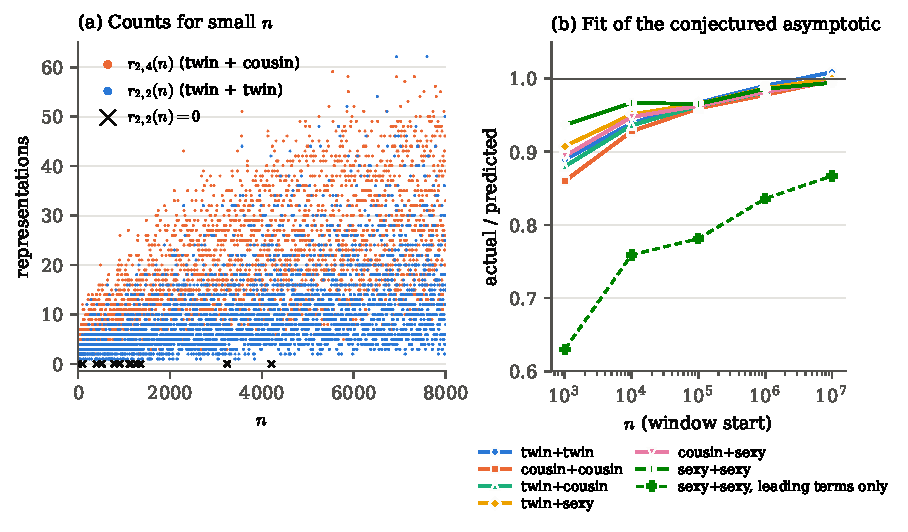
\includegraphics[width=\textwidth]{fig_counts.pdf}
\caption{(a) Unordered counts $r_{2,2}(n)$ (twin $+$ twin) and ordered counts $r_{2,4}(n)$ (twin $+$ cousin) for even $n\le 8000$; crosses mark $r_{2,2}(n)=0$. (b) Mean ratio of actual to predicted counts over the windows of \cref{tab:fit}. The dashed curve uses only the four leading terms for $(6,6)$.}
\label{fig:counts}
\end{figure}

\subsection{Size of the singular series}
On the window $[10^7-2\cdot10^4,10^7)$, the minimum and mean of $\Sg_{a,b}(n)$ are $2.08$ and $6.97$ for $(2,2)$ and $(4,4)$; $4.15$ and $13.94$ for $(2,4)$; and $12.45$, $8.30$, $10.38$ and $27.88$ (common mean) for $(2,6)$, $(4,6)$, $(6,6)$. The twin$+$cousin values are exactly twice the twin$+$twin values. Since the two families have the same density, this factor of two is entirely the symmetry factor $\theta_{2,2}=\tfrac12$. The theorem of \cref{sec:structure} shows that this loss is not merely a matter of counting: for $a=b$ the class $0\bmod3$ loses its second route.

\subsection{Number of exceptions}
Model $r_{a,b}(n)$ as Poisson with mean $\widetilde r_{a,b}(n)$; this is the heuristic suggested by Gallagher's analysis of prime tuples \cite{Gallagher1976}. The expected number of exceptions is then $\sum_n e^{-\widetilde r_{a,b}(n)}$. For $n>1000$ this gives $16.3$ for $(2,2)$ and $16.2$ for $(4,4)$, against $18$ and $19$ observed; $0.19$ for $(2,4)$, against $0$ observed; and less than $0.003$ for each of the three sexy pairings, against $0$. For $n>10^4$ the model gives about $1.0$ for $(2,2)$, while none occur below $10^{11}$ \cite{OEIS_A007534}. This is not a discrepancy. By \cref{cor:triples} exceptions arrive in triples whose members are the same event, so the expected number of exceptional \emph{triples} beyond $10^4$ is roughly half of this sum, and seeing none has probability about $0.6$.

\subsection{Thresholds across gaps}
For each of the $120$ pairs of \cref{tab:grid} we computed $\min\Sg_{a,b}(n)$ over $2\cdot 30030$ consecutive even $n$ near $2\cdot10^6$, a range covering every residue class modulo $2\cdot3\cdot5\cdot7\cdot11\cdot13$, with the products over $\ell$ truncated at $\ell\le200$. The correlation between $\log\min\Sg_{a,b}$ and $\log n_0(a,b)$ is $-0.61$. The singular series explains the coarse ordering. Equal gaps with $3\nmid a$ have the smallest minima ($2.09$ for $a\in\{2,4,8,16\}$, rising to $3.48$ for $a\in\{14,28\}$) and the largest thresholds. For $a=b\in\{10,20\}$ the minimum is $6.26$, larger than the $4.17$ of twin$+$cousin, and the thresholds are small. Pairs with $3\mid ab$ have minima of at least $10.4$. The singular series does not, however, determine individual thresholds. The pairs $(2,4)$ and $(2,16)$ have the same minimum and mean of $\Sg$, yet $n_0=6$ and $n_0=1944$. The Poisson model gives $0.19$ expected exceptions above $1000$ for $(2,4)$; with $120$ pairs, a few late exceptions off the diagonal are to be expected.

\section{Discussion}\label{sec:discussion}

\subsection{On provability}
\Cref{prop:polignac} shows that \cref{conj:main}(1) for any single pair $(a,b)$ implies Polignac's conjecture for gap $a$ or gap $b$. By the work of Zhang, Maynard and the Polymath project \cite{Zhang2014,Maynard2015,Polymath2014}, some gap $d\le 246$ has infinitely many prime pairs, but no specific gap is known to. Even conditionally on strong forms of the Hardy--Littlewood conjectures, the circle method \cite{Vaughan1997} handles binary problems only for almost all $n$, as in \cite{MontgomeryVaughan1975}, not for all large $n$. Inductive arguments face a more basic obstacle. Representability is not hereditary: $4202\in\PP_2+\PP_2$ but $4204\notin\PP_2+\PP_2$. Above $n_0(a,b)$, the inductive step $n\mapsto n+2$ is equivalent to the conjecture itself.

What can be proved is structural. These are the absence of local obstructions (\cref{lem:positivity}), the exact $1:2:1$ locking of equal-gap representations and the two-route phenomenon for distinct gaps (\cref{thm:decomposition} and its corollaries), and the reduction of the twin-prime Goldbach problem for multiples of $6$ to an additive problem for the index set $K_2$ (\cref{cor:index}).

\subsection{Open problems}
\begin{enumerate}
\item Prove that $\{n: r_{a,b}(n)=0\}$ has density zero, conditionally on a suitable form of the Hardy--Littlewood conjectures with uniformity in the shifts.
\item Explain the individual thresholds $n_0(a,b)$, for example the late exception $1942\in E_{2,16}$, beyond the Poisson model.
\item Extend the structure theorem to moduli other than $3$. Congruences $a\equiv\pm b\pmod\ell$ for small primes $\ell\ge5$ may influence $n_0(a,b)$ off the diagonal; for example, $a+b=30$ for $(2,28)$ and $(4,26)$.
\item Study the ternary analogue, sums of three elements of $\PP_a$. Here, too, Vinogradov's method is unavailable without knowing that $\PP_a$ is infinite.
\end{enumerate}

\subsection*{Reproducibility}
The scripts accompanying this paper are \texttt{certify.py} (exact exceptional sets and minimal witnesses), \texttt{hl2.py} (refined prediction $\widetilde r_{a,b}$ and the statistics of \cref{tab:fit}), \texttt{verify\_structure.py} (numerical check of \cref{lem:classes} and \cref{thm:decomposition} for all pairs of gaps in $\{2,4,8,10,14,16,20,22,26,28\}$ up to $10^6$), \texttt{singular\_series\_grid.py} (the correlation across gaps in \cref{sec:evidence}) and \texttt{fig.py} (\cref{fig:counts}). The computed data are included as JSON files.

\bibliographystyle{amsplain}
\bibliography{polignac_goldbach}

\end{document}
